\documentclass[11pt,a4paper]{article}

% Text- und Font-Encoding:
\usepackage[utf8]{inputenc}
\usepackage[T1]{fontenc}

% Worttrennung auf Deutsch:
\usepackage[ngerman]{babel}

\usepackage{listings}

\pagestyle{headings}

% Zeilenabstand
\usepackage{setspace}
\setstretch{1.3}

% Captions
\usepackage[labelsep=newline,labelfont=bf,figurename=Abb.]{caption}
\usepackage{subcaption}
\usepackage[pdftex]{graphicx}

\usepackage{acronym}

% Präambel ende

\begin{document} 


\begin{titlepage}
	\centering
	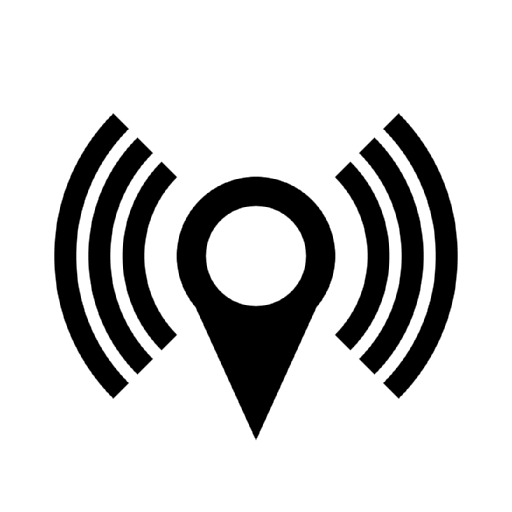
\includegraphics[width=0.25\textwidth]{pics/airsniffer.png}\par\vspace{1cm}
	{\scshape\LARGE Hochschule für Technik und Wirtschaft Berlin \par}
	\vspace{1cm}
	{\scshape\Large Independent Coursework\par}
	\vspace{1.5cm}
	{\huge\bfseries Erfassung und Verabeitung von WLAN Signalen anhand von mobilen Endgeräten für die Nutzung als Positionierungssystem\par}
	\vspace{2cm}
	{\Large\itshape Fabian Bänsch\par}
	\vfill
	betreut von\par
	Prof. Dr. Gefei \textsc{Zhang}

	\vfill

% Bottom of the page
	{\large \today\par}
\end{titlepage}

\tableofcontents{}

\newpage

%TODO WLAN statt WiFi Terminologie

\section{Vorstellung}

Diese Arbeit dient als Dokumentation und Erklärung des Independent Courseworks zum Thema "Erfassung und Verabeitung von WLAN Signalen anhand von mobilen Endgeräten für die Nutzung als Positionierungssystem".

Dieses Verfahren zur Positionsbestimmung mittel WiFi Signalen wird beireits angewandt. Jedoch sind die bisherigen Crowdbasierten Ansätze für die Erstellung solch einer Plattform zu gering vertreten und schwach verbreitet. Die Arbeit soll daher prototyptechnisch diese Thematik untersuchen und am Ende evaluieren.

Es werden dabei verschiedene Softwarekomponenten auf verschiedenen Plattformen für die jeweiligen Aufgabe erstellt. Es wird dabei nur oberflächlich auf die Implementierung eingegangen. Sämtlicher Source Code ist auf GitHub unter der MIT Lizenz veröffentlicht. 
%TODO github + MIT



\section{Konzept}

Mit der Öffnung des Global Postioning Systems (GPS) im Jahre 2000 für die zivile Nutzung war es erstmals für den Endanwender möglich eine Lokalisierung mit einfachen technischen Geräten wie Smartphones zu erreichen.

Das GPS besteht dabei aus einer Reihe an geostationären  Stateliten, welche permanent codierte Radiosignale an die Erde senden. Darin sind der Standort des Sateliten und die genaue Uhrzeit enthalten. Empfangsgeräte können aus diesen Signalen dann ihren Standort mittels der Signallaufzeit errechenen. Eine Sichtverbindung zu mindestens 4 Sateliten wird benötigt.

Dieser Prozess kann entsprechend lange dauern. Das Phänomen wird umgangssprachlich auch "GPS Fix" gennant. Also die verstrichene Zeit, bis das GPS Signal so stabil ist, dass eine Berechnung erfolgen kann. 

Zum anderen hat das globale Positionierungssystem auch Schwächen in stark urbanisierten Bereichen. So ist in Großstädten mit hohen Häusern die Genauigkeit der Berechnung der Position eher schlecht. Dies ist zum einen durch die Verdeckung von Sateliten mit Hochhäusern zu erklären, anderseits kann es auch auch zu Reklektionen von GPS Signalen führen, welche die Positionierung verschlechtern.

Die Idee hinter der WLAN-basierten Ortung gibt es schon bereits seit längerem. Hierbei können Geräte die sichtbaren WLAN Netze in iherer Umgebung an einen zentralen Service senden. Dieser Service kann durch eine Verknüfung von WLAN Netz und Position des Netzes, den Standort des Anfragers errechnen. Dazu muss jedoch der Service über die enstprechenden Daten verfügen. Das heißt, zu sämtlichen Netzen muss der Standort gespeichert sein. Der Aufbau dieser Datenbank stellt dabei eine Sisyphusarbeit dar und muss regelmäßig überholt werden. Anbieter wie Skyhook oder Google 
%TODO REF
nutzen dazu spezielle Fahrzeuge mit Messantennen, welche durch die Städte fahren (Meist in Verbindung mit anderen Aufgaben). 
%TODO Streeview oa.

Daneben gibt es auch solche Services, welche auf Crowdbasierte Informationen zurückgreifen. Dabei kann jeder einen Beitrag leisten und so zum Aufbau, Erweiterung und Wartung des Services beitragen. Als Beispiel seien hier Wigle oder OpenWifi.su. genannt.
%TODO REF
Als primärer Verwendungszweck des hier vorgestellten Projekts soll eben dieser Crowd-basierte Ansatz sein.

Im weiteren Verlauf der Arbeit wird daher zunächst nocheinmal ein Blick auf raumbezogene Daten geworfen und inwiefern dies verarbeitet werden können. Danach folgt eine allgemeiner Abriss über das Anwendungsdesign und aller Komponenten des Systems. 

In den folgenden Kapiteln wird dann zunächst erläutert wie WLAN Daten gesammelt werden, diesen dann einer zentralen Einheit (API) zugestellt wird und mittels einer Visualierung bzw der Standortbestimmung seitens des Endanwenders benutzt werden kann

%TODO Warchalking
%TODO Sniffer vs. API vs. Locator vs. Visualisierung (Grob)

\section{Geospatial Data}

Dieses Kapitel gibt eine kurze Einführung un raumbezogene Daten, wie mit dieses gerechnet werden kann und wie eine Interpolation für das hier vorgestellte System durchgeführt wird.

Raumbezogene Daten auf der Erde können auf verschiedenen Arten angegeben werden. Hierbei wird die Erde als Kugel betrachtet und entsprechend können Kugelkoodinaten als Ortsbestimmung benutzt werden. Dazu werden 180 Breitengrade (horizontal) und 360 Längengrade (vertikale) erstellt. Ein Punkt auf der Erde kann nun mit nur 2 Angaben eindeutig bestimmt werden. Der speziellen Längen und Breitengrade. Klassischerweise wird dabei zu verfeinerung mit Stunden, Minuten und Sekunden gearbeitet. Da Computer eher schlecht ein Basis 60 System zu Berechnung nutzen können, kann die Unterteilung auch dezimal erfolgen. Dies wird hier auch der Fall sein. 

Um die Distanz von 2 Punkten berechnen zu können wird die harversine Distanz verwendet. Sie stellt sicher, dass die Krümmung der Erde bei der Distanzberechnung mit berücksichtig wird~\cite{harversine_distance}.

\begin{lstlisting}[language=Java]
public static final double R = 6372.8; // In kilometers
public static double haversine(
		double lat1, 
		double lon1, 
		double lat2, 
		double lon2) {
    double dLat = Math.toRadians(lat2 - lat1);
    double dLon = Math.toRadians(lon2 - lon1);
    lat1 = Math.toRadians(lat1);
    lat2 = Math.toRadians(lat2);
    double a = Math.pow(Math.sin(dLat / 2),2) +
    	Math.pow(Math.sin(dLon / 2),2) * 
    	Math.cos(lat1) * Math.cos(lat2);
    double c = 2 * Math.asin(Math.sqrt(a));
    return R * c;
}
\end{lstlisting}
%TODO REF

Da wir später an mehreren Orten das WLAN Signal eines Routers einfangen werden, stellt sich die Frage, wie können wir auf den Quellort des Signals schließen. Hier gibt es mehrere Verfahren. Ich werde zu Beginn lediglich den Durchschnitt der Koordinaten als Zentrum benutzen. In späteren Versionen kann dort noch ein Gewichtung mit der Qualität des GPS und der aktuellen Empfangsleistung des WLANs kombiniert werden.

\section{Anwendungsdesign}

Das System wird sich wie eingangs erwähnt in 4 Teile untergliedern, welche voneinander losgelöst arbeiten können.

Der ''\textbf{AirSniffer}'' ist die Smartphone Anwendung, welche für das Sammeln der Daten zuständig ist. Diese muss dabei so gestaltet werden, dass zunächst keine API Anbindung notwendig ist. Sie soll autark - also offline - ebenso funktionieren. Daher muss hier eine Datenbank zur Speicherung der lokalen Ergebnisse stattfinden. Diese Resultate können dann an die API gesendet werden, um die Daten zu veröffentlichen. Als Prototyp wird eine Anwendung in Android (nativ) umgesetzt. 

Die ''\textbf{AirPI}'' dient als zentaler Service des Systems. Hier können die Daten der AirSniffer App hochgeladen werden. Zudem werden Funktionalitäten zum Abrufen der WLAN bzw. raumgebundenen Daten angeboten, welche die verarbeitenden Apps nutzen können. Die API wird unter Python mit Flask laufen. Für den Datenhaushalt sorgt eine MongoDB.

Die ''\textbf{AirVis}'' Anwendung dient als Visualisierungtool der Daten aus der AirPI. Die webbasierte Anwendung stellt dabei eine interakive Karte mit verschiedenen Filterfunktion zur Verfügung. Daraus können aus den Rohinformation ein positiver Mehrwert gezogen werden. Technolgien für die Umsetzung sind dabei HTML, Javascript und CSS. Zudem wird die Google Maps API verwendet. Aufgesetzt wird die Anwenudung in einer Linux / Apache Umgebung.

Der ''\textbf{AirLocator}'' ist eine beispielhafte Anwendung, welche auf Grundlage der Daten aus der API eine Positionsbestimmung durchführt. Die eigentliche Berechnung wird dabei von der AirPI ausgeführt. Die Anwendung dient lediglich als Anzeige. Wie auch der AitSniffer wird sie als native Android API mit einer Google Maps API Anbindung programmiert.

Alle Komponenten in ihren Beziehung ist in Abbildung~\ref{fig:Anwendungsdesign} ersichtlich.

\begin{figure}[htbp]
    \centering
    \begin{subfigure}[b]{1\textwidth}
        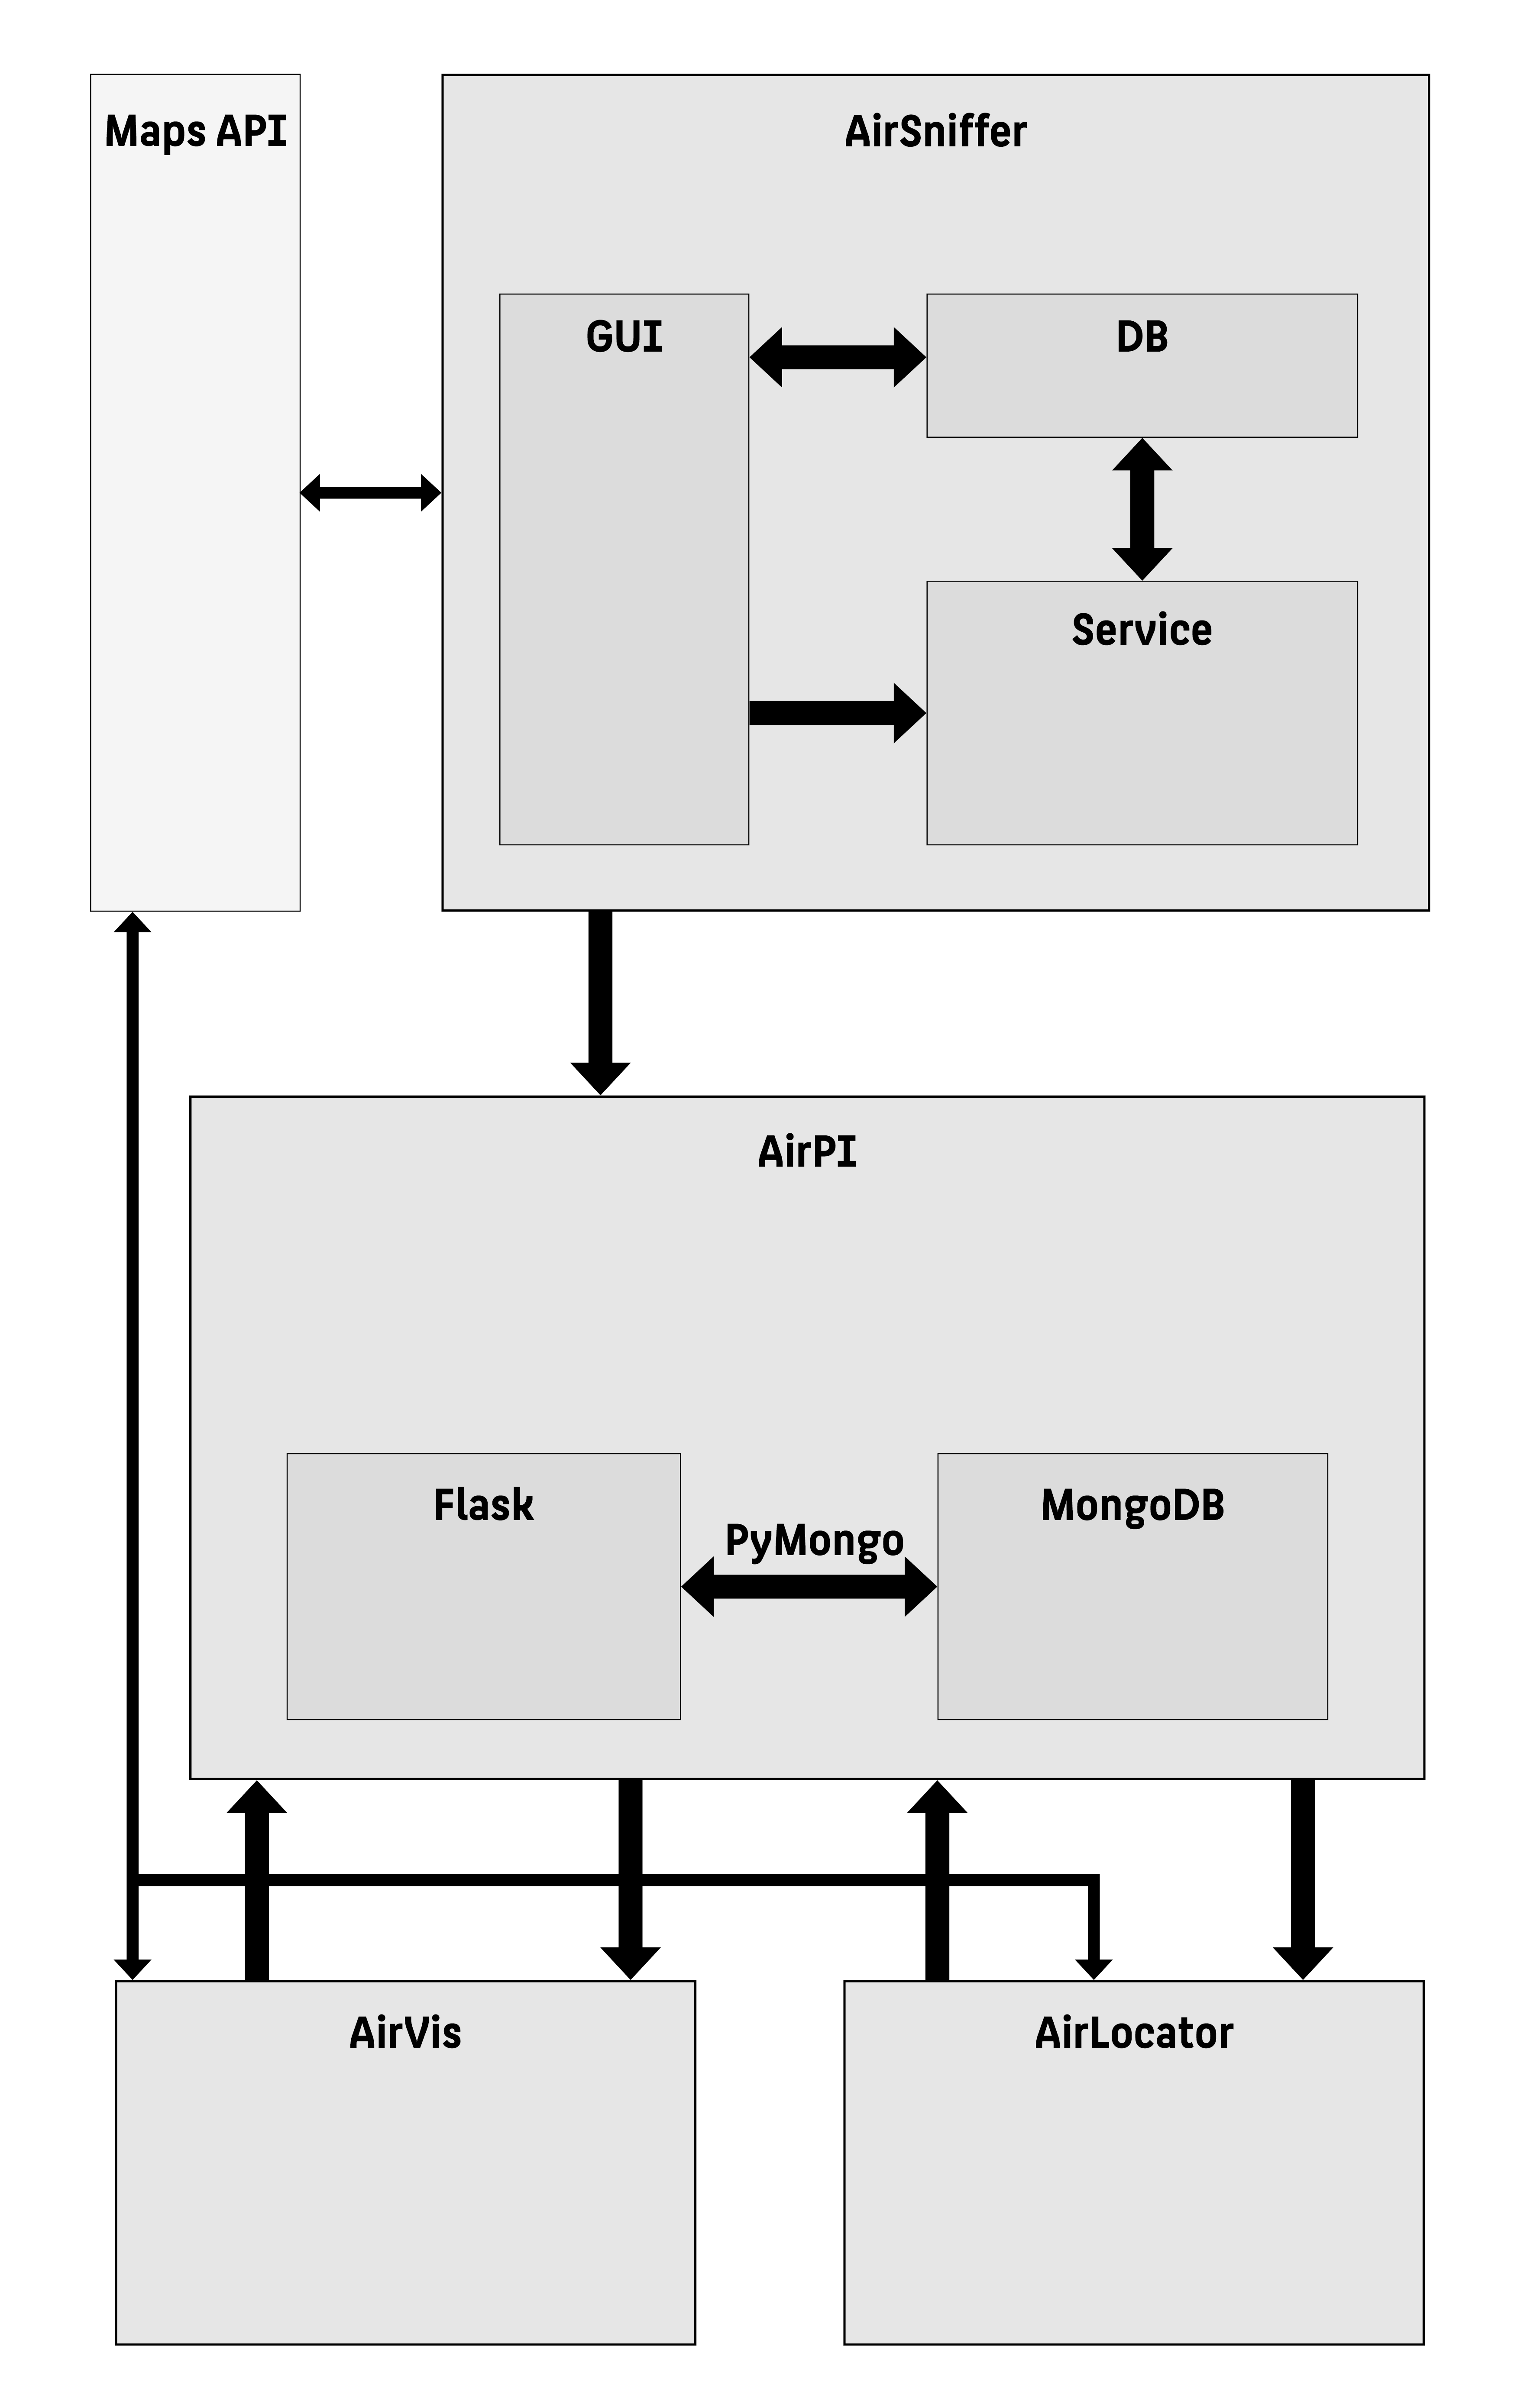
\includegraphics[width=\textwidth]{pics/AirAndwenungsdesign.png}
    \end{subfigure}
    \caption{Anwendungsdesign}\label{fig:Anwendungsdesign}
\end{figure}

\newpage
\section{AirSniffer}

Als Datemerfassungsandwendung wurde wie einfangs der AirSniffer entwickelt. Dies ist eine App unter Android. Sie soll dabei autark von der API breits laufen können, und ähnliche Funktionalitäten aufweisen. Dazu musste zunächst eine Datenbank auf dem Endgerät erstellt werden, um die aufgespührten Netzwerke persistent abszuspeichern. Android bietet dazu eine relationelle SQLite Datenbank an. Für den Andwendungsfall hier haben dabei 2 Tabellen gereicht. Eine für die WLANs und eine zur Speicherung der Örtlichkeeit. Dabei entsteht eine 1:n Beziehung. Das heißt, ein Gerät kann meherere Örtlichkeiten haben. Die Örtlichkeiten stellen dabei die Orte dar, an dem das Netzwerk sichtbar war. Die  Struktur der Datenbank sieht entsprechend wie folgt aus:

\begin{figure}[htbp]
    \centering
    \begin{subfigure}[b]{1\textwidth}
        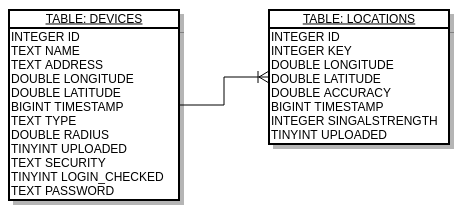
\includegraphics[width=\textwidth]{pics/dbView.png}
    \end{subfigure}
    \caption{Datenbankmodell}\label{fig:DB_VIEW}
\end{figure}

Der Key aus der ''Locations'' Tabelle dient dabei als Fremdschlüssel für den Eintrag aus ''Devices''. Jeder ''Device'' Eintrag hat zudem selber ein Feld mit der Angabe zur Längen- und Breitengrad. Hier wird später der Mittelwert errechnet und eingetragen. Dies dient lediglich der Perfomancestreigerung. 

Um das Protokollieren von WLAN Daten im Hintergrund ausführen zu können, wurde eine selbständiger Service implementiert. Dieser ist unabhängig von der App. Die App mit den GUI Elementen kann diesen lediglich starten und stoppen. Daraus ergeben sich jedoch auch folgende Vorteile: Der Background Service erhält mehr Rechenleistung, er kann auch bei nichtaktiver GUI weiterarbeiten. Als wichtigister Vorteil ist jedoch, dass der Service nicht abbrechbar seitens Android ist. Normalerweise unterbricht Android nebenläufige Hintergrundprozesse nach einer gewissen Zeit. Ebenso kann der Prozess auch nicht beenedet werden, wenn der Benutzter die App absichtlich versucht zu stoppen. 

Nachteilig ist jedoch, dass die Kommunikation von GUI und Backgroundservice nicht mehr einfach herzustellen ist. Daher wurde für GUI Anwendung lediglich auf die Einträge der Datenbank zurückgegriffen.

Das Mitlesen der Nachrichten findet nun im Backgroundservice statt. Hier können verschiedene Sniffer Instanzen gestartet werden
\footnote{Es gibt Sniffer für WLAN Netze, Bluetooth Low Energy Geräte und Bluetooth EDR Geräte. Hier in der Arbeit wird primär auf den Einsatz der WLAN Netze eingegangen}.
Das Mitlesen von derzeitig verfügbaren WLAN Netzen unter Android kann wie im folgenden Codebeispiel angeregt werden.

\begin{lstlisting}[language=Java]
String connectivityContext = Context.WIFI_SERVICE;
final WifiManager wifiManager = (WifiManager) getContext()
   .getSystemService(connectivityContext);
if (wifiManager.isWifiEnabled()) {
   wifiManager.startScan();
}
\end{lstlisting}

Die Callbacks werden typischerweise unter Android mit einem Broadcastreceiver aufgefangen. Notwendiger müssen diese zunächst angemeldet werden. Ein beispielhafter Broadcastreceiver sieht wie im folgenden Codebeispiel aus:

\begin{lstlisting}[language=Java]
BroadcastReceiver receiver = new BroadcastReceiver() {
   @Override
   public void onReceive(Context context, Intent i) {
      WifiManager wm = (WifiManager) context
      .getSystemService(Context.WIFI_SERVICE);
      List<ScanResult> results = wm.getScanResults();
      for (ScanResult scanResult : results) {
         String ssid = scanResult.SSID;
      }
   }
};
\end{lstlisting}

Diese Scanresults werden dann adaptiert auf ''Device'' Modell und zusätzlich mit den aktuellen Koordinaten versehen. Um die Performace zu steigern wurde auch eine Senke als Thread erstellt, welche für das weitere Handling zuständig ist. Hier wird beim Versuch das neue Geräte der Datenbank hinzuzufügen zunächst geschaut, ob es bereits enthalten ist. Ist dies der Fall, so werden lediglich die neuen Koordinaten als weiteren Ort hinzugefügt
\footnote{Dabei werden noch weitere Berechnungen durchgeführt. Zum Beispiel muss ein Mindestabstand von 2m zwischen verschiedenen Orten gewährleistet sein. Es werden zusätzlich die Daten auf Richtigkeit geprüft. So ist ein sehr schlechtes GPS Signal zum Beispiel nicht weiter verwendbar und der Eintag wird verworfen}.
Im Folgenden weiteren weitere Information hinzugefügt. So wird einer neuer Mittelpunkt des Netzes sowie sein Radius berechnet. Im Falle eines neu entdeckten Netzes wird auch eine Notification samt Vibration an das Android OS gesendet.
%TODO REF TO Screenshot.

Die eigentliche App mit sämtlichen GUI Elementen ist wie oben beschrieben unabhängig von dem eigentlichen Sniffen. Hier gibt es verschiedene Views, welche auch teilweise die Google Maps API verwenden.
So gibt es zunächst eine Listenansicht mit allen lokal gesnifften Netzen. Ein Indikator gibt an, ob es sich um ein WLAN, BL LE oder BL EDR Gerät handelt. Zudem kann man auch direkt nach Netzen suchen. Die Detailansicht eines Gerätes offenbart zusätzlich alle referenzierte Orte, an den das Gerät sichtbar war. 
Beide Views können dabei auch als Kartenansicht gestartet werden. Dabei wird zum Beispiel auch der Radius visualisert. 

Sämtliche Informationen sind jedoch lokal erstellt und stammen vom eigenem Gerät. Daher stellt die Anwendung auch eine Logik zum Hochladen sämtlicher gesnifften Netze an die AirPI zur Verfügung. Hierbei wird auf das Json Format zurückgegriffen. 

Es hat sich unter Android gezeigt, dass es keine Suche seitens des Betriebssystems gibt, wenn der Bildschirm in den Ruhezustand geht. Daher wurde eine zusätzliche View erstellt, welche als Sperrbilschirm dient und den Bildschirm nicht abschaltet.

%TODO wificracker anteasern

\section{AirPI}

Dieser Teil des Systems soll als zentrales Rückrat dienen. Hier können ersniffte Netze hochgeladen und gespeichert werden. Zudem sollen weitere Prozeduren entahlten sein, um diese zu optimieren und zu validieren. 
Des weiteren sollen Schnittstellen gefunden werden, um die vorhanden Daten sinnvoll  verschiedene Services anzubieten.

Technisch wurde hier aus einer Kombination von Flask und MongoDB mit PyMongo als Bindeglied gesetzt. Flask ist ein Webframework unter Python. Enthalten ist eine Template Enging ''Jinja2'' und die hier benötigte Bibliothek ''Werkzeug'' zum erstellen von WSGI Anwendungen (Web Server Gateway Interface). Flask ist sehr handlich. Die Hello World Anwendung besteht aus gerade mal 7 Zeilen Code.

\begin{lstlisting}[language=Python]
from flask import Flask
app = Flask(__name__)

@app.route("/")
def hello():
    return "Hello World!"
    
if __name__ == "__main__":
    app.run()
\end{lstlisting}
%TODO REF http://flask.pocoo.org/

\noindent Zusätliche wurde eine Basic Authentifizierung eingeführt. Diese ist mit einem statischen Benutzer und Kennwort vorgegeben.
Mit dieser Vorgehensweise wurden folgende API Signaturen erstellt. 

\begin{lstlisting}[]
GET     /devices
POST	/devices
GET     /devicesAtPos
GET     /devicesAtRect
GET     /device
GET     /status
GET     /alive
GET     /location
\end{lstlisting}

Die MongoDB Datenbank ist eine Dokumentbasierte Datenbank. Daher kann die relationale Datenbank aus Android nicht einfach auf diese gemappt werden. Stattdessen ist nun die ''Locations'' Tabelle, welche via Fremdschlüssel angesprochen wurde, direkt als Set im ''Device'' Modell enthalten. Dies stellt auch automatisch sicher, dass keine Duplikate von Orten enthalten sein kann.

Die MongoDB wird nicht direkt angesprochen, sondern mit den PyMongo Wrapper. Hier lassen sich nach erfolgreichen Instanzierung aber auch normale MongoDB Queries starten. Beispiel sieht das wie im folgenden Codebeispiel aus:

\begin{lstlisting}[language=Python]
from flask_pymongo import PyMongo
app.config['MONGO_DBaddress'] = 'db'
app.config['MONGO_URI'] = 'mongodb://localhost:27017/db'
mongo = PyMongo(app)
devices = mongo.db.devices.find()
for device in devices:
   app.logger.info(str(device))
\end{lstlisting}

Hier werden lediglich alle ''Devices'' aus der Datenbank geladen und via dem Logger ausgegeben. 
Ein großer Vorteil von MongoDB ist das Arbeiten mit dem Geospitial-Index, welcher direkt angeboten wird. Dadurch kann die MongoDB höchstperfomant eine Reihe an Daten liefern, welche zum Beispiel innerhalb einer gegeben Bounding Box liegen. Dazu ein Codebeispiel:

\begin{lstlisting}[language=Python]
mongo.db.devices.create_index([("loc", GEO2D)])
query = [{"loc": {"$within": {"$box": [
   [swLon, swLat], [neLon, neLat]]
   }}}]
devices = mongo.db.devices.find({"$and": query}
\end{lstlisting}
%TODO ensureInddex vs createÍndex


\newpage
\noindent
Im folgenden werden einige Routen mit deren Funktionalitäten vorgestellt.

\begin{itemize}
\item{} \textbf{GET /devices}

Hier werden alle Devices geliefert, welche den Typen aus der Parameterliste übereinstimmen. Diese Route ist nur für Testzwecke und für die Anbindung an andere Services gedacht. 
%TODO welche Services - dieses github dingens?!

\item{} \textbf{POST /devices}

Das Hinzufügen von neuen Geräten aus der AirSniffer Applikation wird über diese Route gehandhabt. Die entsprechenden Geräte müssen im Body des Requests als Json vorliegen. Im nachhinein findet noch eine Optimierung satt. Das bedeutet, zu nah aneinanderliegende Orte werden entfernt sowie der Berechnung von einem neuen Mittelpunkt und dem Radius.

\item{} \textbf{GET /devicesAtPos}

Mittels des Geospitial-Index werden hier alle Geräte geliefert, welche an einem Ort und deren Umkreis liegen. Diese Daten werden als Query Parameter mit übergeben.

\item{} \textbf{GET /devicesAtRect}

Ähnlich der vorherigen Route. Nur kann hier eine Bounding Box angegeben werden.

\item{} \textbf{GET /device}

Weitere Informationen zu einem Gerät inklusive aller vorhanden Orte bei denen das Gerät erkundet wurden, werden hier geliefert. Als Identikiationsmittel wird die MAC Adresse des Gerätes via Query Parameter mit hineingereicht.

\item{} \textbf{GET /location}

Diese Route berechnet anhand von gegeben MAC Adressen den mittleren Standort. Die Adressen werden im Request Body als Json mit übergeben. Anhand des mittleren Standorts der Geräte kann im folgenden eine Positionsbestimmung eines Clients durchgeführt werden.

\end{itemize}

%TODO Dependencies
%TODO Installationsanleitung
%TODO Beispiel GET mit Request

\section{AirVis}

AirVis ist die Visualisierungkomponente in diesem System. Sie ist webbasiert und ermöglicht die Veranschaulichung der in der AirPI gespeichert Daten. Durch das einfache Navigieren mittels einer Karte und verschiedenen Filterungstechniken entsteht ein erheblicher Mehrwert für den Nutzer.

Die verwendeten Techniken sind im groben HTML, Javascript in Kombination mit der Google Maps API und des eigens entwickelten AirPI. Als Grundfunktion steht zunächst eine Kartenansicht wie auch auf maps.google.de zu sehen ist. Im Weiteren wird diese jedoch mit den gesnifften Netzen aus der AirPI angereichert. Dazu wird der jeweilige Kartenausschnitt als Bounding Box erfasst und an die AirPI gesendet. Wie aus dem vorherigen Kapitel bereits beschrieben, werden nun alle Netze in dieser Box aggregiert und an den Client zurückgesendet. Diese Daten werden dann vom Webclient mittels einfacher Marker auf die Map gesetzt.

Durch Klick auf einen dieser Marker werden dabei zusätzliche Informationen zu diesem Netz von der AirPI abgerufen. So erscheinen nun zusätzliche alle referenzierte Orte zu diesen Netz.

Somit können mit diesen einfachen Mitteln bereits die Welt nach Netzwerken erkundet werden. Zusätzlich wurde ein Filterpanel integriert. Hier kann z.B. gezielt nach einem Netz gesucht werden oder aber verschiedene Typen von Netzen an- und ausgeschaltet werden
\footnote{Unterscheidung nach WLAN, BL LE und BL EDR}.
Ebenso is es möglich nach Parametern wie Aznahl referenzierter Orten oder Größe des Radius zu filtern. 

Ein Statuspanel zeigt überdies die Anzahl der verschiedenen Elemente in der AirPI an sowie die Zeiten der AirPI bei der Beantwortung von verschieden Requests.

\section{AirLocator}

Der AirLocator ist eine Applikation unter Android, welche einen praktischen Nutzen aus des ganzen Daten ziehen soll. Dabei soll wie in der Vorstellung beschrieben eine Positionsbestimmung rein durch das Wissen von umgebenen WLAN Netzen möglich sein. 

Als Vorleistung dazu wurde bereits der AirPI mit der Route GET /Location ausgestattet, welche im Body des Requests eine Json Datei erwartet mit verschiedenen WLAN Netzen. Daraus errechnet sie mit den vorhandenen Daten eine Position und schick diese zurück. Das heißt, der AirLocator braucht lediglich die stark abgeschwächte Funktionalität des AirSniffers (Das Scannen nach umliegenden WLAN Netzen).

Die Sniffer Funktionalität konnte dabei fast komplett übernommen werden. Nur werden die Daten nicht in eine Datenbank abgespeichert, sondern via eines HTTP GET an den AirPI gesendet. Im Gegenzug erhalten wir dann den errechneten Längen- und Breitengrad. 

Dazu wurde in der Applikation lediglich ein GUI ELement erstellt. Eine View mit der Karte aus der Google Maps API. Bei erfolgreichem Response wird diese Position mittels Marker auf die Karte dargestellt. Es wird dabei jede Sekunde nach WLAN Netzen geschaut und ein Request gestartet. Um die Veränderungen der Position sichtbar zu machen, wurde zudem eine Spur in Form eines blauen Pfades der Map hinzugefügt. 

\section{Auswertung}

%TODO Zeitmessung - Airlocators
%TODO Zeitmessung - API Request mit BoundingBox 
%TODO Always On Screen
%TODO Genauigkeit der ermittelten WLAN Spots
%TODO Genauigkeit der Messung (Airlocator)
%TODO Genauigkeit GPS

\section{Fazit}

%TODO Ziel erreicht
%TODO Skaliebarkeit fragwürdig
%TODO --> Clustering
%TODO was ist mit den ganzen gesnifften Bluetooth Dingern?
%TODO Zusammenwirken mit anderen Apps (Navigation etc.)

\section{Ausblick}

%TODO Offline Rendering der Map
%TODO what todo with BL?
%TODO Other Stuff doable with all the data
%TODO Different DB for different Typs
%TODO Clustering of DB
%TODO Multithreading of API


\newpage
\section{Abkürzungsverzeichnis}

\begin{acronym}
 \acro{GPS}		{Global Positioning System}
 \acro{WLAN}	{Wireless Local Area Network} 
 \acro{API}		{Application Programming Interface}
 \acro{HTTP}	{Hypertext Transfer Protocol}
 \acro{JSON}	{JavaScript Object Notation}
 \acro{REST}	{Representational State Transfer}
 \acro{FQDN}	{Fully Qualified Domain Name}
 \acro{DNS}		{Domain Name System}
 \acro{CPU}		{Central Processing Unit}
 \acro{WSGI}	{Web Server Gateway Interface}
 \acro{BL LE}	{Bluetooth Low Energy (Bluetooth 4)}
 \acro{BL EDR}	{Bluetooth Enhanced Data Rate (Bluetooth 2)} 
\end{acronym}


\begin{thebibliography}{99}

\bibitem{nyt} The New York Times Developer Network, https://developer.nytimes.com/

\bibitem{unlock_slider} Stack Overflow - Wow to make slide to unlock button in Android, https://stackoverflow.com/questions/14910226

\bibitem{harversine_distance} Harversine Distanz, 
https://rosettacode.org/wiki/Haversine\textunderscore formula

%TODO ICONS 8

\end{thebibliography}


\end{document}
